\section{Sprint 4}

\subsection*{Summary}

\begin{table}[H]
	\centering
	\begin{tabular}{ll}
		\toprule
		\multicolumn{2}{c}{\textbf{Sprint 4}}\\
		\midrule
		\textbf{Periode} & 30.03.2015 12:00 Uhr\textendash 13.04.2015 12:00 Uhr\\
		\textbf{Stunden Soll} & \SI{144}{\hour}\\
		\textbf{Stunden Plan} & \SI{134}{\hour} \\
		\textbf{Stunden Ist} & \SI{134.5}{\hour}\\
		\bottomrule
	\end{tabular}
\end{table}

\begin{figure}[H]
	\centering
	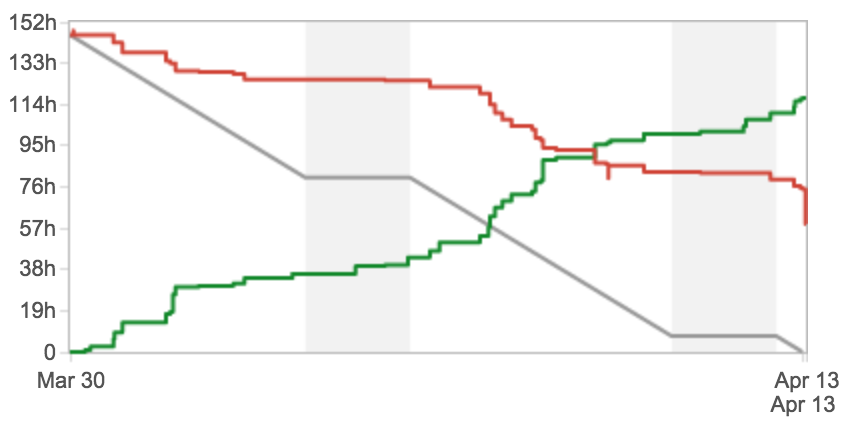
\includegraphics{fig/bd-sprint-4}
	\label{fig:pm:bd-sprint-4}
	\caption*{Burndown Chart Sprint 4}
\end{figure}

\subsection*{Ziele}
Das Hauptziel dieses Sprints liegt in der Entwicklung der Schema-Transformationssprache. Der Favorit zu Beginn des Sprints war die Verwendung eines eigenen SQL Dialekts. Die Vor- und Nachteile verschiedener Lösungen wurden evaluiert.

\subsection*{Abgeschlossen}
Folgende High-level (ohne Subtasks) Jira Tasks wurden während Sprint 4 abgeschlossen. 

\begin{table}[H]	
\centering
\begin{tabular}{ll}
	\toprule
	\textbf{JIRA-Key} & \textbf{Summary}\\
	\midrule
DAT-74 & Übrige Aufwände Sprint 4\\
DAT-75 & Organisation, Planung \& Kommunikation Sprint 4\\
DAT-76 & Projektmeetings Sprint 4\\
DAT-78 & Basis Transformationen	Story\\
DAT-79 & Transformation erstellen\\
	\bottomrule
\end{tabular}	
\end{table}

Ein SQL Subset/Dialekt ``\acs{odhql}'' mit SQL-Basisfunktionalität (Selektion, Joins, Bedingungen, Funktionen) und einige String- und Geometriefunktionen wurden implementiert. Weitere Funktionen werden bei Bedarf hinzugefügt. Das User-Interface (DAT-79) ist noch im Anfangsstadium und wird in den nächsten Sprint weiterentwickelt.

\subsection*{Probleme}
Minimale Koordinationsprobleme durch die unterrichtsfreie Zeit über Ostern. Teammitglied \rlif hat viel Zeit durch Ausfall seiner Entwicklungsumgebung und dessen Neuinstallation verloren.
